\documentclass[a4paper,12pt]{article}

\usepackage{tikz}
\usepackage[utf8]{inputenc}
\usepackage[english]{babel}
\usepackage{amssymb,amsmath,amsthm}

\newtheorem{theorem}{Theorem}
\newtheorem{example}{Example}
\newtheorem{problem}{Problem}
\newtheorem{lemma}{Lemma}

\usepackage{mathtools} % Bonus
\DeclarePairedDelimiter\norm\lVert\rVert

\title{Feb 25 Lecture}
\author{COMP2804 Winter 2020}

\begin{document}

\section{Monte Hall Problem}
  - 3 doors and they contain 2 goats, 1 sports car \\ 
  - You pick a door at random. It stays closed \\ 
  - Monte opens one the other two doors and shows you a goat (always). \\ 
  - You can have what's behind your current door or the other (unopened)  door. \\
  - $S = \{Car, Goat\#1, Goat\#2 \}$ \\
  - $Pr(w) = 1/3 \text{ for each w} \in S.$\\ 
  - A = "You picked the door with the car"\\
  - $Pr(A) = \frac{1}{3}$ \\
  - $Pr(A^\complement) = 1 - Pr(A) = 2/3$\\
\subsection{example}
  - Anil has two children, $S = \{bb,gg,bg,gb\}$\\
  - At least one of Anil's children is a boy\\
  - $B = \{bb,bg,gb\}$\\
  - What is the probability that both of Anil's children are boys\\
  - $A = \{bb\}$\\
  - $Pr(A) = \frac{1}{3}$\\ 
Definition: Let (S, Pr) be a probability space are $A, B \subseteq S$ 
be events with $Pr(B) > 0$ then 
\begin{center}
    $$Pr(A | B) = \frac{Pr(A \cap B)}{Pr(B)}$$
\end{center}
This is telling the \textit{"probability of A given B."} \\ 
\begin{center}
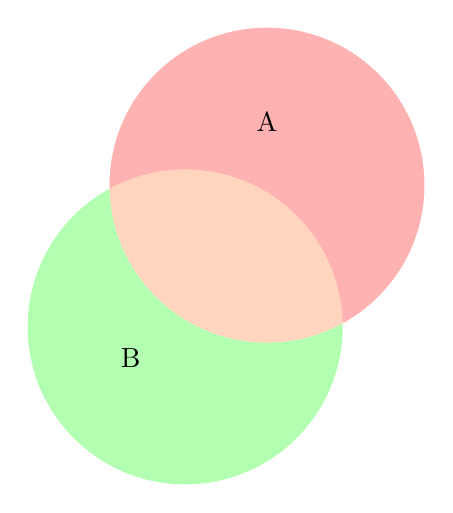
\begin{tikzpicture}
    \begin{scope}[blend group = soft light]
    \fill[red!30!white]   ( 90:1.2) circle (2);
    \fill[green!30!white] (210:1.2) circle (2);
    \end{scope}
    \node at ( 90:2)    {A};
    \node at ( 210:2)   {B};
    \node [font=\small] {};
\end{tikzpicture}
$$Pr(A) = \frac{Pr(A)}{Pr(S)}$$ In the universial set S
\end{center}
Now we can compute the probability of Anil's children 
\begin{align*}
    Pr(A | B) &= \frac{Pr(A \cap B)}{Pr(B)} \\ 
    &= \frac{Pr(bb)}{3/4}  = \frac{1/4}{3/4}\\
    &= 1/3 
\end{align*}
Roll a die $S = \{1,2,3,4,5,6\} Pr(w) = 1/6$ for each $w \in S$\\
A = "the result of the roll is 3" $= \{3\}$. $Pr{A} = 1/6$ \\
B = "the result is an odd integer" $= \{1,3,5\}$ $Pr{B} = \frac{B}{S}$ \\
\begin{align*}
    \Pr(A | B) &=  \frac{Pr(A \cap B)}{Pr(B)} \\ 
    &= \frac{Pr(\{3\})}{1/2} = \frac{1/6}{1/2} = 2/3 \\ 
    &= 1/3
\end{align*}
\begin{align*}
    Pr((B|A)^\complement) &= \frac{Pr(A\cap B)}{Pr(A)} \\ 
    &= \frac{Pr(\{3\})}{Pr(\{3\})} = 1   
\end{align*}
C = "the result is a prime number" $= {2,3,5}$\\ 
\begin{align*}
    Pr(C|B) &= \frac{Pr(B \cap C)}{Pr(B)} \\ 
    &= \frac{Pr(\{3,5\})}{3/6} = \frac{2/6}{3/6} = 2/3  
\end{align*}
$B^{\complement}$ = "The result is an even integer \{2,4,6\}.
\begin{align*}
    Pr(C|B^{\complement}) &= \frac{Pr(C \cap B^{\complement})}{Pr(B)} \\ 
    &= \frac{Pr(\{2\})}{3/6} = \frac{1/6}{3/6} = 1/3  
\end{align*}
\begin{lemma}
    $$Pr(A | B) + Pr(A^\complement | B) = 1$$
\end{lemma}
\textbf{Def.}
\begin{align*}
    Pr(A | B) + Pr(A^\complement | B) &= \frac{Pr(A\cap B) + Pr(A^\complement \cap B)}{Pr(B)} 
\end{align*}
(missed some )\\ 
 - Anil has two children \\ 
 - At least one of Anil's children is a boy who was born on a Sunday.\\ 
 - What is the probability that both of Anil children are boys \\
$S = \{(s_{1}, d_{1}, s_{2}, d_{2} ): s_{1}, s_{2} in \{b,g\} d_{1}, d_{2} \in W \}$\\
$W = \{Su, Mo, Tu, Thur, Fri, Sat\}$\\
$|S| = 14^2$\\
$|W| = 7$\\
$B=$ "At least one of Anil's children is a boy who was born on a Sunday."
$A=$ "both Anil's children are boys."\\ 
$B = \{(b,Su, s_{2},d_{2}): s_{2}\in\{b,g\}, d_{2} \in W\} \cup \{(s_{1}, d_{1}, b, Su): s_{1}\in\{b,g\}, d_{1} \in W\}$\\
$A = \{(b_{1}, d_{1}, b_{2}, d_{2}): d_{1}, d_{2} \in W\}$\\ 
$A \cap B = \{(b,Su, b,d_{2}):  d_{2} \in W\} \cup \{(b, d_{1}, b, Su): d_{1} \in W\}$\\
$|A \cap B| = |X \cup Y|$\\ 
$|A \cap B| = |X| + |Y| - |X \cap Y| = 7 + 7 - 1 = 13$\\
$|B| = |X^{'} \cup Y^{'}|$\\ 
$|B| = |X^{'}| + |Y^{'}| - |X^{'} \ cap Y^{'}| = 14 + 14 - 1 = 27$\\

\begin{align*}
    \Pr(A | B) &=  \frac{Pr(A \cap B)}{Pr(B)} \\ 
    &= \frac{Pr(|A\cup B| \setminus |S|)}{Pr(|A\cup B| \setminus |S|)}\\
    &= \frac{13}{27}\\ 
    &= 48.15\% ???!?!
\end{align*}
\end{document}